\documentclass[a4paper, 12pt]{article}
\usepackage[a4paper,top=1.5cm, bottom=1.5cm, left=1cm, right=1cm]{geometry}
\usepackage{cmap}					
\usepackage{mathtext} 				
\usepackage[T2A]{fontenc}			
\usepackage[utf8]{inputenc}			
\usepackage[english,russian]{babel}
\usepackage{multirow}
\usepackage{graphicx}
\usepackage{wrapfig}
\usepackage{tabularx}
\usepackage{float}
\usepackage{longtable}
\usepackage{hyperref}
\hypersetup{colorlinks=true,urlcolor=blue}
\usepackage[rgb]{xcolor}
\usepackage{amsmath,amsfonts,amssymb,amsthm,mathtools} 
\usepackage{icomma} 
\usepackage{euscript}
\usepackage{mathrsfs}
\usepackage{enumerate}
\usepackage{caption}
\usepackage{enumerate}
\mathtoolsset{showonlyrefs=true}
\usepackage{graphicx}
\usepackage{caption}
\usepackage{subcaption}
\usepackage{amsthm}
\usepackage[europeanresistors, americaninductors]{circuitikz}
\DeclareMathOperator{\sgn}{\mathop{sgn}}
\newcommand*{\hm}[1]{#1\nobreak\discretionary{}
	{\hbox{$\mathsurround=0pt #1$}}{}}

\title{\textbf{Определение $\displaystyle C_p/C_v$ по скорости звука в газе (2.1.3)}}
\author{Манро Эйден}
\date{}

\begin{document}

\maketitle

\begin{center}
    \section*{Введение}
\end{center}

    \noindent \textbf{Цель работы:} 1) измерение частоты колебаний и длины волны при резонансе звуковых колебаний в газе, заполняющем трубу; 2) определение показателя адиабаты с помощью уравнения состояния идеального газа.\hfill

    \bigskip

    \noindent \textbf{Оборудование:} звуковой генератор; электонный осциллограф; микрофон; телефон; раздвижная труба; теплоизолированная труба, обогреваемая водой из термостата; баллон со сжатым углекислым газом.
 

    \bigskip

\begin{center}
    \section*{Теоретические сведения}
\end{center}

\begin{equation} \label{velocity}
    c=\sqrt{\gamma\frac{RT}{\mu}}
\end{equation}

\bigskip

где $ R $ -- газовая постоянная, $ T $ -- температура газа, а $ \mu $ -- его молярная масса. Преобразуя эту формулу, найдем:

\bigskip

\end{equation}
\begin{equation}\label{gamma}
    \gamma = \frac{\mu}{RT}c^2
\end{equation}

\bigskip
    
Таким образом, для определения показателя адиабаты достаточно измерить температуру газа и скорость распространения звука (молярная масса газа предполагается известной).
    
Звуковая волна, распространяющаяся вдоль трубы, испытывает многократные отражения от торцов. Звуковые колебания в трубе являются наложением всех отраженных волн и очень сложны. Картина упрощается, если длина трубы $ L $ равна целому числу полуволн, то есть когда

\bigskip

\begin{equation} \label{lambda}
    L=\frac{n \lambda}{2}    
\end{equation}

\bigskip

где $ \lambda $ -- длина волны звука в трубе, а $ n $ -- любое целое число. Если это условие выполнено, то волна, отраженная от торца трубы, вернувшаяся к ее началу и вновь отраженная, совпадает по фазе с падающей. Совпадающие по фазе волны усиливают друг друга. Амплитуда звуковых колебаний при этом резко возрастает -- наступает резонанс.

При звуковых колебаниях слои газа, прилегающие к торцам трубы, не испытывают смещения. Узлы смещения повторяются по всей длине трубы через $ \lambda/2 $. Между узлами находятся максимумы смещения.

Скорость звука c связана с его частотой $ f $ и длиной волны $ \lambda $ соотношением

\bigskip

\begin{equation}\label{lambda_f}
c=\lambda f
\end{equation}

\bigskip
\newpage

Подбор условий, при которых возникает резонанс, можно производить двояко:

\begin{enumerate}
\item При неизменной частоте $ f $ звукового генератора (а следовательно, и неизменной длине звуковой волны $ \lambda $) можно изменять длину трубы $ L $. Для этого применяется раздвижная труба. Длина раздвижной трубы постепенно увеличивается, и наблюдается ряд последовательных резонансов. Возникновение резонанса легко наблюдать на осциллографе по резкому увеличению амплитуды колебаний. Для последовательных резонансов имеем
\item 
\begin{equation}\label{first}
L_n=n\frac{\lambda}{2}, \quad L_{n+1}=(n+1)\frac{\lambda}{2}, \quad \dots, \quad L_{n+k} = n\frac{\lambda}{2}+k\frac{\lambda}{2},
\end{equation}
 т. е. $ \lambda/2 $ равно угловому коэффициенту графика, изображающего зависимость длины трубы $ L $ от номера резонанса $ k $. Скорость звука находится по формуле \eqref{lambda_f}.
\item При постоянной длине трубы можно изменять частоту звуковых колебаний. В этом случае следует плавно изменять частоту $ f $ звукового генератора, а следовательно, и длину звуковой волны $ \lambda $. Для последовательных резонансов получим 
\begin{equation}\label{4}
L=\frac{\lambda_1}{2}n=\frac{\lambda_2}{2}(n+1)=\dots=\frac{\lambda_{k+1}}{2}(n+k).
\end{equation}

Из \eqref{lambda_f} и \eqref{4} имеем:
\[ f_1=\frac{c}{\lambda_1}=\frac{c}{2L}n, \quad f_2=\frac{c}{\lambda_2}=\frac{c}{2L}(n+1)=f_1+\frac{c}{2L},\quad \dots, \]
\begin{equation}\label{5}
f_{k+1}=\frac{c}{\lambda_{k+1}}=\frac{c}{2L}(n+k)=f_1+\frac{c}{2L}k.
\end{equation}
Скорость звука, деленная на $ 2L $, определяется, таким образом, по угловому коэффициенту графика зависимости частоты от номера резонанса.
\end{enumerate}

\begin{center}
\subsection*{Экспериментальная установка}
\end{center}

Соответственно двум методам измерения скорости звука в работе имеются две установки (рис. \ref{img1} и \ref{img2}). В обеих установках звуковые колебания в трубе возбуждаются телефоном Т и улавливаются микрофоном М. Мембрана телефона приводится в движение переменным током звуковой частоты; в качестве источника переменной ЭДС используется звуковой генератор ГЗ. Возникающий в микрофоне сигнал наблюдается на осциллографе ЭО.

Микрофон и телефон присоединены к установке через тонкие резиновые трубки. Такая связь достаточна для возбуждения и обнаружения звуковых колебаний в трубе и в то же время мало возмущает эти колебания: при расчетах оба торца трубы можно считать неподвижными, а влиянием соединительных отверстий пренебречь.

Первая установка (рис. \ref{img1}) содержит раздвижную трубу с миллиметровой шкалой. Через патрубок (на рисунке не показан) труба может наполняться воздухом или углекислым газом из газгольдера. На этой установке производятся измерения $ \gamma $ для воздуха и для $ CO_2 $. Вторая установка (рис. \ref{img2}) содержит теплоизолированную трубу постоянной длины. Воздух в трубе нагревается водой из термостата. Температура газа принимается равной температуре омывающей трубу воды. На этой установке измеряется зависимость скорости звука от температуры.

\begin{figure}[H]
    \begin{center}
        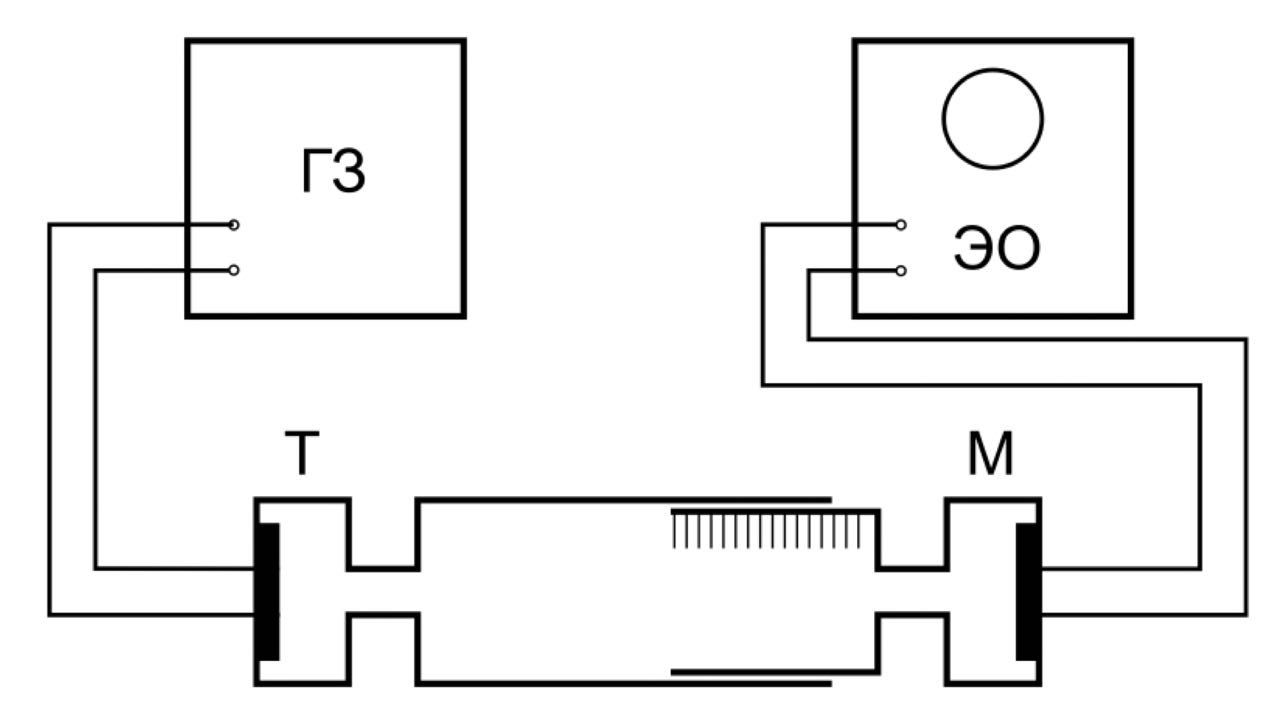
\includegraphics[width=12cm]{ust1.jpg}
    \end{center}
    \caption{Установка для измерения скорости звука при помощи раздвижной трубы}
    \label{img1}
\end{figure}

\begin{figure}[H]
    \begin{center}
        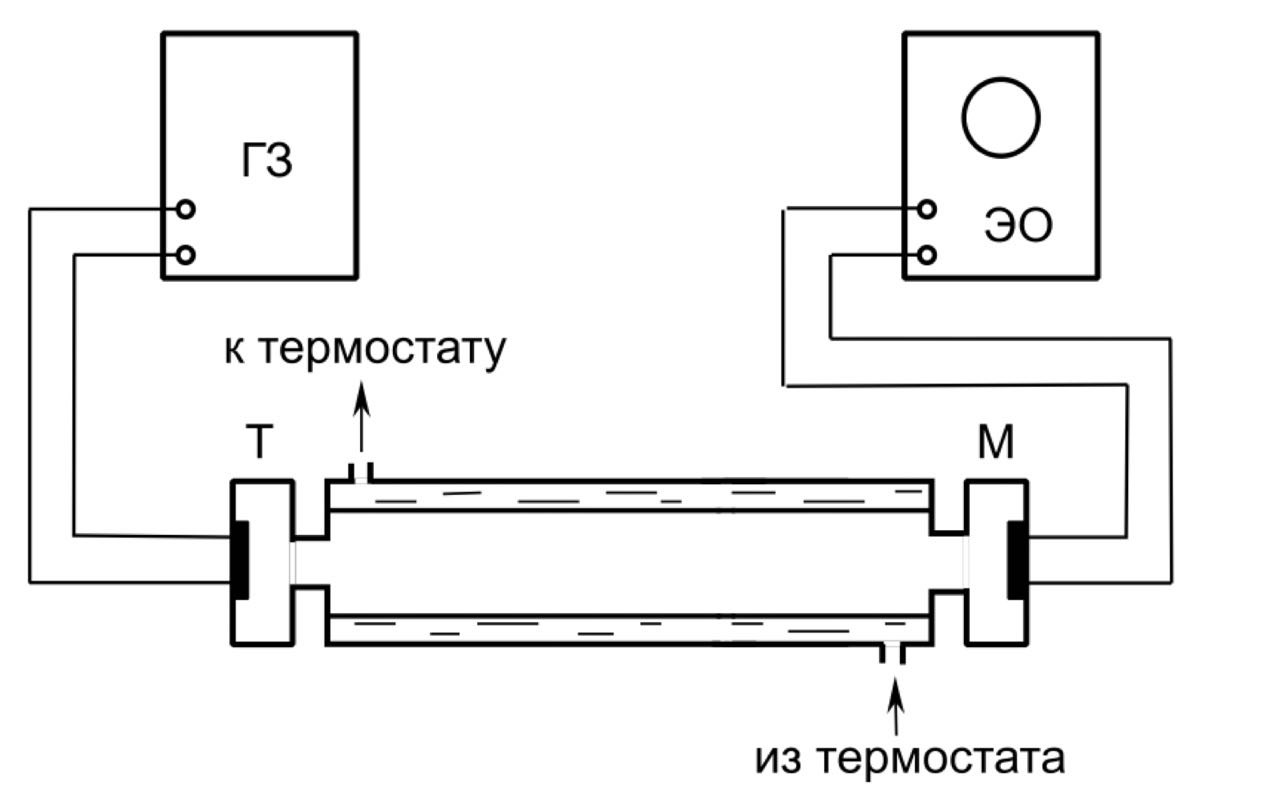
\includegraphics[width=12cm]{ust2.jpg}
    \end{center}
    \caption{Установка для изучения зависимости скорости звука от температуры}
    \label{img2}
\end{figure}

\begin{center}
    \subsection*{Погрешности}
\end{center}

\begin{itemize}
    \item $\sigma_t = 0,2 \; ^{\circ}$ C
    \item $\sigma_L = 1 \; \text{мм}    $
    \item $\sigma_\nu = 2 \; \text{Гц}$
    \item \text{МНК аппроксимация с помощью компьютера}
\end{itemize}

\newpage

\begin{center}
    \section*{Ход работы}
\end{center}

Проведём измерение коэффициента $ C_p/C_v $ для воздуха при помощи установки с раздвижной трубой. Для проведения серии измерений фиксируем частоту звукового сигнала и оставляем её неизменной до окончания снятия показаний. Увеличиваем и уменьшаем длину трубки, чтобы добиться резонанса, возникновение которого устанавливается при помощи осциллографа. При возникновении резонанса фиксируем то расстояние, на которое была выдвинута трубка прибора. Данные измерения проводим для нескольких значений частот. Полученные результаты заносим в таблицу 1. Все измерения проводились при температуре в комнате $t_0=(21,9 \pm 0,2) \; ^{\circ} C$

\bigskip

\begin{table}[h]
    \begin{center}
        \begin{tabular}{|p{2cm}|p{2cm}|p{2cm}|p{2cm}|p{2cm}|p{2cm}|}
            \hline
            \multicolumn{6}{|c|}{$CO_2$, $L = (575 \pm 5)$ мм} \\ \hline
            $ n $ & 1 & 2 & 3 & 4 & $\nu$, \text{Гц} \\ \hline
            $\Delta L_1$, мм & 230 & 181 & 84 & 40 & 2700 \\ \hline
            $\Delta L_2$, мм & 229 & 180 & 82 & 38 & 2690 \\ \hline
            $\Delta L_3$, мм & 228 & 179 & 81 & 37 & 2685 \\ \hline
        \end{tabular} \label{oxy}
        \caption {Увеличение длины трубы при резонансе} 
    \end{center}
    \end{table}

\bigskip

Средняя погрешность измеренной длины составила $\sigma_L\approx 1$ мм.

По данным таблицы 1 построим график \ref{fig:CO} зависимости удлинения трубы от номера полученного резонанса, считая первое удлинение соответствующим первому резонансу (вычитание константы не меняет наклон графика).

\begin{figure}[H]
	\begin{center}
		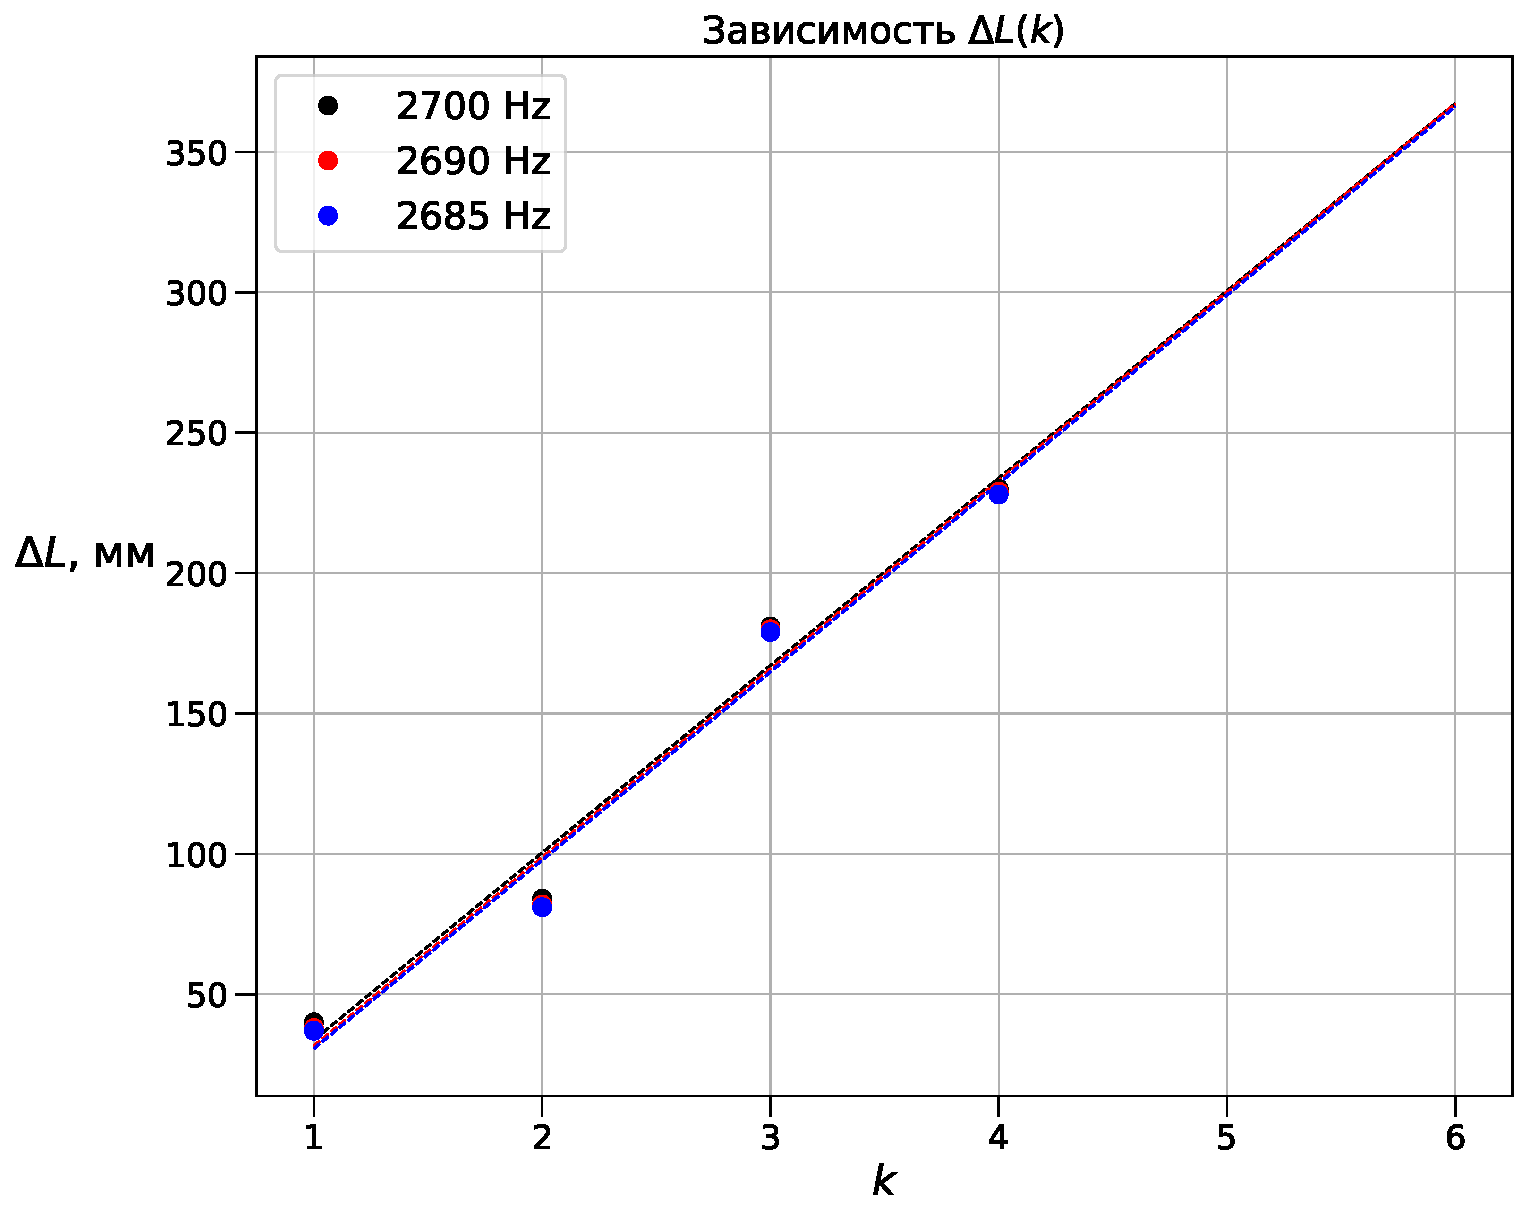
\includegraphics[scale=0.60]{CO.pdf}
		\caption{\centering График зависимости удлинения трубы \\ от номера полученного резонанса для $CO_2$}
		\label{fig:CO}
	\end{center}
\end{figure}

Из графика и формул, приведенных выше, находим, что скорость углекислого газа равна:

\begin{equation}
    c_{CO_2} = (274,2 \pm 4,2) \; \text{м/c}
\end{equation}

И соответственно находим показатель адиабаты:

\begin{equation}
    \gamma_{CO_2} = (1,35 \pm 0,05) \; \text{м/с} 
\end{equation}

Проведём измерения $ C_p/C_v $ для воздуха при различных температурах. Для этого будем использовать трубу постоянного размера $L = (700 \pm 1)$ мм. Для фиксированной температуры будем изменять частоту звукового сигнала, тем самым изменяя и длину волны, так, чтобы мы могли наблюдать последовательные резонансы. Для каждого резонанса будем фиксировать частоту, при которой он возник. Полученные измерения занесём в таблицу 2.

\bigskip

\begin{table}[h]
    \begin{center}
    \begin{tabular}{|p{2cm}|p{2cm}|p{2cm}|p{2cm}|p{2cm}|p{2cm}|}
    \hline
    \multicolumn{2}{|c|}{$t=20^\circ C$} & \multicolumn{2}{|c|}{$t=40^\circ C$} & \multicolumn{2}{|c|}{$t=55^\circ C$} \\ \hline
    $n$ & $\nu_{\text{рез}}$, \text{Гц} & $n$ & $\nu_{\text{рез}}$, \text{Гц} & $n$ & $\nu_{\text{рез}}$, \text{Гц} \\ \hline
    1 & 260  & 1 & 268  & 1 & 275  \\ \hline
    2 & 497  & 2 & 511  & 2 & 523  \\ \hline
    3 & 739  & 3 & 760  & 3 & 779  \\ \hline
    4 & 985  & 4 & 1015 & 4 & 1038 \\ \hline
    5 & 1230 & 5 & 1268 & 5 & 1297 \\ \hline
    \end{tabular}
    \label{tab:constL}
    \end{center}
    \caption {\centering Результаты измерений резонансной частоты при разных температурах и числу полуволн}
\end{table}

Максимальная погрешность измеренной частоты оказалась равной $\sigma_{\nu}\approx2$ Гц.

\begin{figure}[H]
	\begin{center}
		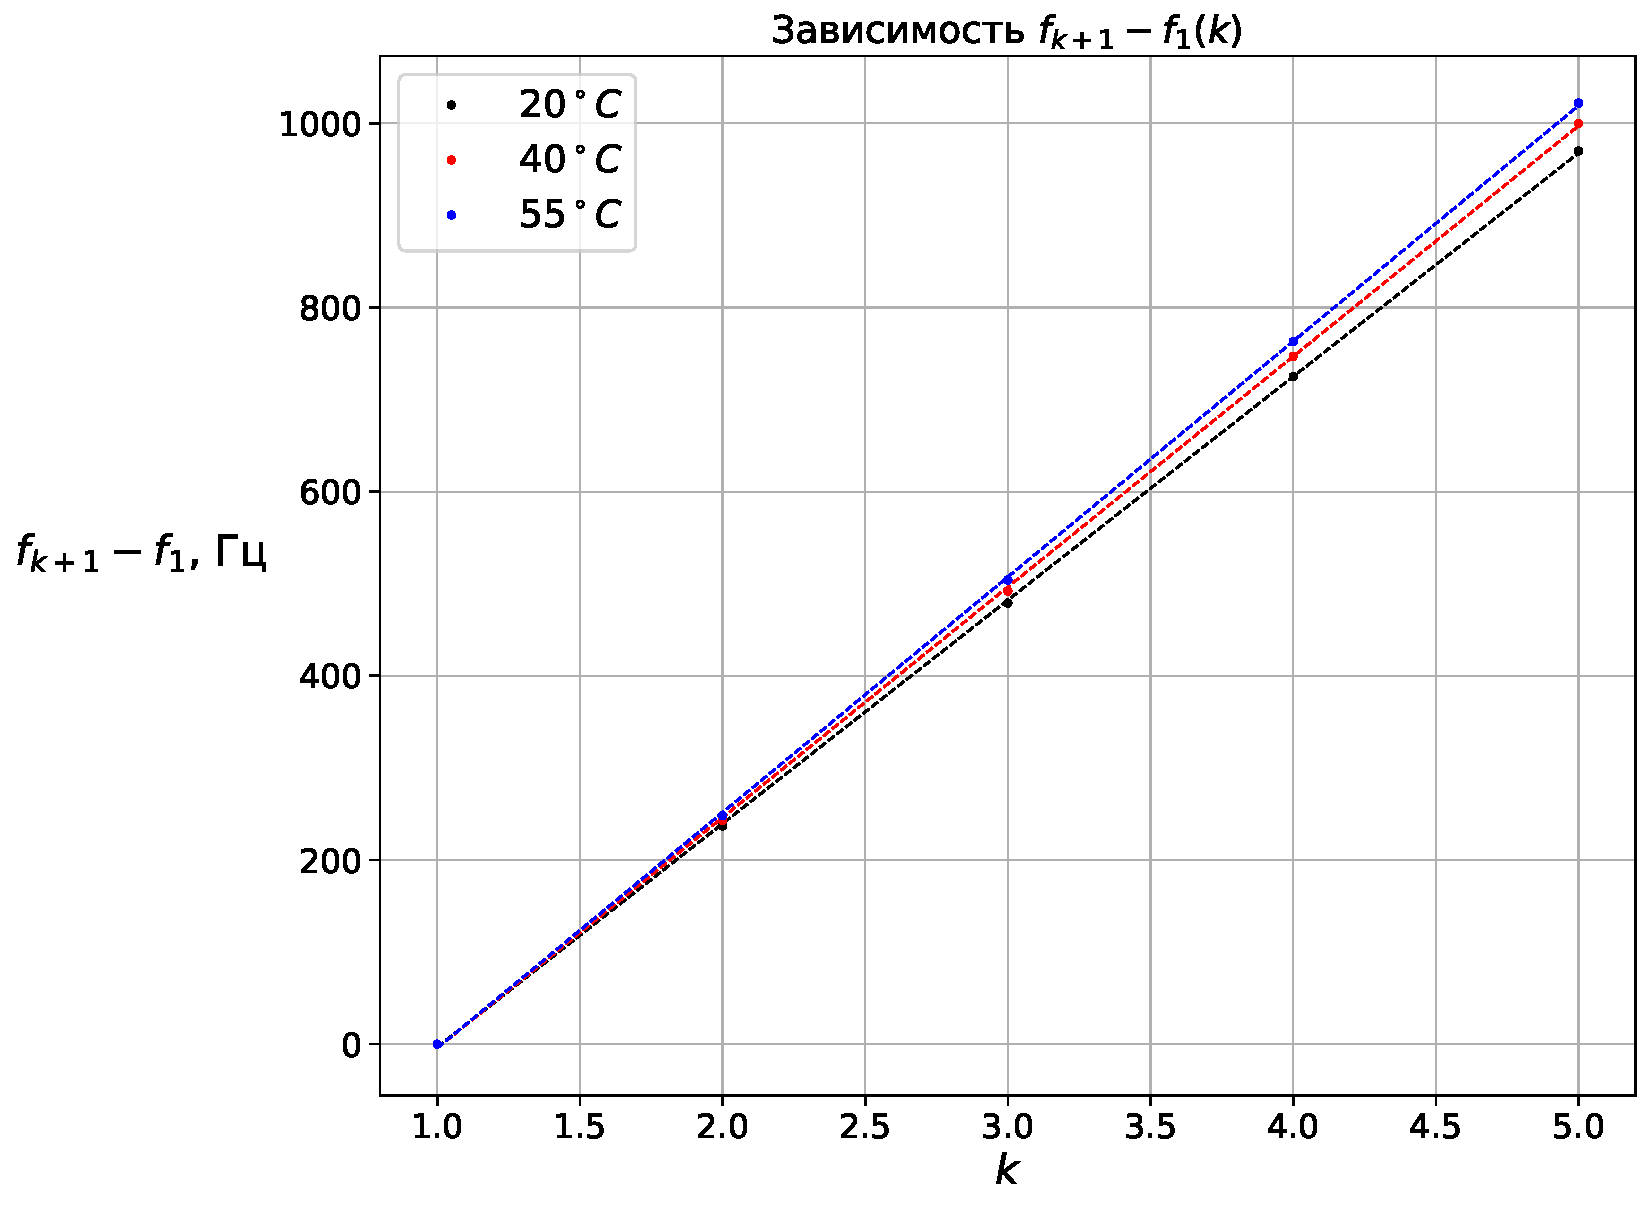
\includegraphics[scale=0.6]{nu(k).pdf}
		\caption{График зависимости $f_{k+1} - f_1$ от номера резонанса при различных температурах}
		\label{nu(k)}
	\end{center}
\end{figure}

По наклону графика найдём скорость звука для каждой температуры:

\begin{center}
    $\displaystyle c_{20}=(339,9 \pm 1,0)$ м$/$с 
    \break
    
    $\displaystyle c_{40}=(350,5 \pm 1,4)$ м$/$с 
    \break
    
    $\displaystyle c_{55}=(358,2 \pm 1,3)$ м$/$с 
    \break
\end{center}

По формуле \eqref{gamma} найдём $\displaystyle C_p/C_v$:

\begin{center}
    
    $\displaystyle \gamma_{20}=1,37 \pm 0,02$
    \break
    
    $\displaystyle \gamma_{35}=1,39 \pm 0,02$
    \break
    
    $\displaystyle \gamma_{50}=1,36 \pm 0,03$
    \break
\end{center}

\begin{center}
    \section*{Обсуждение результатов}
\end{center}

Измерения проводились на установке, на которой длина трубы оставалась постоянной на протяжении всего опыта, а резонанса мы добивались при помощи изменения частоты звукового сигнала. В ходе этих измерений также исследовалась зависимость коэффициента адиабаты $ \gamma $ от температуры газа. Было получено, что показатель адиабаты не зависит от температуры в диапазоне температур $ 20-60 $ $ ^\circ C $ и равняется:

\[ \boxed{\gamma_{\text{воздух}} = 1,37 \pm 0,02}\quad\]

Сравним полученные данные с табличными. Согласно справочнику, показатель адиабаты для воздуха при нормальных условиях равен \underline{$ \gamma = 1,4 $}. Таким образом, можно утверждать, что результат измерения $ \gamma $ на первой установке в пределах погрешности совпадает с табличными данными. Результаты измерения на второй установке незначительно отличаются от табличных. Это может быть связано с большой неточностью определения резонансных частот на второй установке. Чтобы этого избежать, необходимо использовать генератор частоты с возможностью более точной настройки для возможности чёткого отслеживания резонансов.

Также в ходе работы был измерен показатель адиабаты для углекислого газа. Измерения проводились на первой установке. В итоге мы получили \[ \boxed{\gamma_{CO_2} = 1,35\pm 0,05}\quad\]

Сравним эти данные с табличными. Согласно справочнику, показатель адиабаты для углекислого газа при нормальных условиях \underline{$ \gamma = 1,3 $}. Таким образом, полученные данные незначительно отличаются от табличных. Это может быть связано с тем, что при измерениях в трубе находился углекислый газ с примесями (в основном, азот и кислород), которые могли исказить результаты измерений. Для повышения точности, эксперимент стоит проводить в атмосфере углекислого газа, чтобы исключить попадание различных примесей в трубу.

\begin{center}
    \section*{Выводы}
\end{center}

В ходе выполнения работы мы:

\begin{itemize}
	\item измерили частоту колебаний и длину волны при резонансе звуковых колебаний в газе, заполняющем экспериментальную установку;
	\item определили разными методами показатель адиабаты с помощью уравнения состояния идеального газа.
\end{itemize}


\end{document}
